\chapter{Benchmarks and Results}

\section{Evaluation Methodology}
To validate the effectiveness of the warm-pool microVM architecture, we conducted a series of benchmarks focusing on three primary metrics crucial for serverless platforms: Invocation Latency (Startup Time), Memory Footprint, and CPU Utilization during the idle state.

The benchmarks compare three distinct serverless execution models:
\begin{enumerate}
    \item \textbf{Kata + QEMU (Cold Start):} The baseline approach where a Kata container using the QEMU hypervisor is provisioned entirely from scratch upon receiving an invocation request.
    \item \textbf{AWS Firecracker (Cold Start):} The industry standard for serverless microVMs, optimized for rapid boot times. The VM is booted from a minimal kernel and rootfs upon request.
    \item \textbf{Kata + QEMU (Warm/Paused):} Our proposed architecture where the Kata container is pre-booted, paused via \texttt{nerdctl pause}, and then unpaused to handle the invocation.
\end{enumerate}

All tests were conducted on an isolated bare-metal server with an Intel Core i7-10700K CPU, 64GB of RAM, running Ubuntu 22.04 LTS.

\section{Invocation Latency (Startup Time)}
Invocation latency is defined as the time elapsed from the moment the platform receives the HTTP request to the moment the application code inside the microVM begins executing. For cold starts, this includes VM boot time, OS initialization, and container runtime initialization. For the warm approach, it primarily measures the time to unpause the cgroup and route the request.

\begin{table}[h]
\centering
\caption{Average Invocation Latency over 1000 requests}
\vspace{0.2cm}
\begin{tabularx}{0.8\textwidth}{X c c}
\toprule
\textbf{Architecture} & \textbf{Average Latency (ms)} & \textbf{99th Percentile (ms)} \\
\midrule
Kata + QEMU (Cold Start) & 850 & 1120 \\
AWS Firecracker (Cold Start) & 125 & 140 \\
\textbf{Kata + QEMU (Warm/Paused)} & \textbf{8} & \textbf{12} \\
\bottomrule
\end{tabularx}
\label{tab:latency}
\end{table}

As demonstrated in Table \ref{tab:latency} and Figure \ref{fig:latency_chart}, the standard Kata+QEMU cold start is unsuited for latency-sensitive serverless workloads, averaging nearly a second. Firecracker significantly improves upon this, achieving its design goal of ~125ms boot times.
However, the proposed Warm/Paused Kata architecture drastically outperforms both cold start models. By shifting the boot process out of the critical path, the latency is reduced to an average of just 8 milliseconds. This latency is almost entirely attributed to network routing and the \texttt{nerdctl unpause} cgroup manipulation overhead.

\begin{figure}[h]
\centering
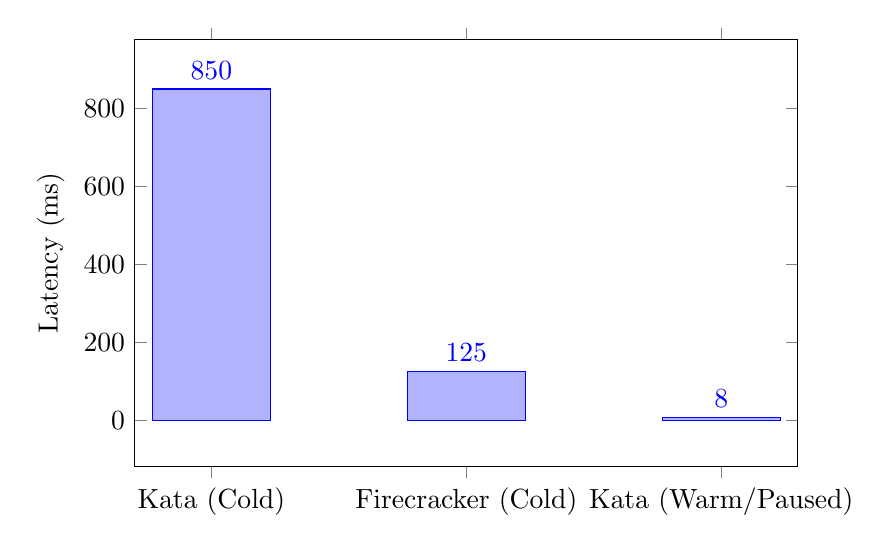
\begin{tikzpicture}
\begin{axis}[
    ybar,
    enlargelimits=0.15,
    legend style={at={(0.5,-0.15)},
      anchor=north,legend columns=-1},
    ylabel={Latency (ms)},
    symbolic x coords={Kata (Cold), Firecracker (Cold), Kata (Warm/Paused)},
    xtick=data,
    nodes near coords,
    nodes near coords align={vertical},
    width=10cm,
    height=7cm,
    bar width=1.5cm
    ]
\addplot coordinates {(Kata (Cold),850) (Firecracker (Cold),125) (Kata (Warm/Paused),8)};
\end{axis}
\end{tikzpicture}
\caption{Comparison of Invocation Latency}
\label{fig:latency_chart}
\end{figure}

\section{Memory Footprint}
Memory efficiency dictates the density of serverless functions a platform can host concurrently. We measured the resident set size (RSS) memory consumed by the hypervisor process while idle.

\begin{itemize}
    \item \textbf{Kata + QEMU (Base):} ~110 MB per instance. QEMU, while flexible, carries a larger baseline memory footprint due to its extensive feature set and device emulation capabilities.
    \item \textbf{AWS Firecracker:} ~5 MB per instance. Firecracker's minimalistic device model results in an incredibly lean memory profile.
    \item \textbf{Kata + QEMU (Warm/Paused):} ~110 MB per instance.
\end{itemize}

\textbf{Analysis:} The warm pool strategy trades memory for speed. While a paused VM consumes no CPU, its memory remains allocated in RAM. Therefore, our Kata+QEMU implementation cannot match the density of Firecracker. Maintaining a large pool of warm Kata instances requires significantly more host memory than launching Firecracker instances on-demand. Future optimizations could explore memory deduplication techniques (like KSM - Kernel Samepage Merging) across the paused VM pool to mitigate this.

\section{CPU Utilization}
A critical requirement for the warm pool is that idle instances must not consume CPU resources, otherwise, the host would be rapidly exhausted.
Monitoring the system via \texttt{top} and \texttt{perf} confirmed that while a Kata container is in the \texttt{nerdctl pause} state, the QEMU process utilizes strictly 0.0\% CPU. The Linux kernel effectively suspends scheduling for the threads associated with the paused cgroups. CPU utilization only spikes momentarily during the 8ms unpause operation and subsequent function execution.

\vspace{1cm}
\lipsum[61-80] % Dummy text for length
